Here we derive the Laplacian of a feed-forward neural network with scalar output, that is $\Delta u_{\vtheta} \coloneqq \Tr(\gradsquared{\vx} u_{\theta})$.
The goal is to make the dependence of the Laplacian w.r.t.\,a weight $\mW$ in one layer of the network explicit.
Then we can write down the Jacobian $\jac_{\mW}(\Delta u_{\vtheta})$ which is required for the Fisher used by energy NGD.

We first lay out the notation for feedforward neural networks, then use the ideas of Hessian backpropagation \citep[HBP,][]{dangel2020modular} to derive a recursion for the Hessian $\gradsquared{\vx}u_{\vtheta}$.
The Laplacian follows by taking the trace of the latter.
Finally, we express the Laplacians gradient w.r.t.
a single layer's weight $\mW$, i.e.\,$\nicefrac{\partial \Delta u_{\vtheta}}{\partial \mW}$, in terms of $\mW$'s children in the compute graph.

%\subsection{Feed-forward Neural Networks}
\paragraph{Layer notation} Consider a sequential neural network $u_{\vtheta}$ with depth $L$ that consists of layers $f^{(i)}_{\vtheta^{(i)}}$ with trainable parameters $\vtheta^{(i)} \in \sR^{d^{(i)}}, i=1,\dots, L,$ that transform an input $\vx \in \sR^M$ into a prediction $u_{\vtheta}(\vx)\in \sR^C$ via intermediate representations $\vz^{(i)} \in \sR^{h^{(i)}}, i= 0, \dots, L$,
\begin{align}
  \begin{split}
    u_{\vtheta}
    &=
      f^{(L)}_{\vtheta^{(L)}} \circ f^{(L-1)}_{\vtheta^{(L-1)}} \circ \ldots \circ f^{(1)}_{\vtheta^{(1)}}
    \\
    f^{(i)}_{\vtheta^{(i)}}\colon \sR^{h^{(i-1)}}
    &\to
      \sR^{h^{(i)}}\,,
    \\
    \vz^{(i-1)}
    &\mapsto
      \vz^{(i)} = f^{(i)}_{\vtheta^{(i)}}(\vz^{(i-1)})
  \end{split}
\end{align}
where $\vz^{(0)} \coloneqq \vx$, $\vz^{(L)} \coloneqq \vu$, and $\vtheta = ({\vtheta^{(1)}}^{\top}, \dots, {\vtheta^{(L)}}^{\top})^{\top}$ is the concatenation of parameters over layers.
A parameter might be empty, e.g.\,if the layer is an activation layer.



%\subsection{Derivatives}

\paragraph{Flattening} Above, we assumed all quantities ($\vz^{(i)}, \vtheta^{(i)}$) to be vectors.
In case of tensor-valued quantities, we can first flatten them into vectors to reduce to the vector case.
Our index convention to vectorize will be first-varies-fastest, which means column-stacking for a matrix (row index varies first, column index varies second).
We denote the flattening operation by $\flatten(\cdot)$.
Very useful is the so called \emph{vec-trick} stating that 
\begin{equation}\label{eq:vecTrick}
    \flatten(AXB) = (B^\top\otimes A)\flatten{X}
\end{equation}
for matrices $A, X, B$. In particular, this shows that $B^\top\otimes A$ is the  matrix representing the linear mapping $X\mapsto AXB$ and hence $J_X(AXB) = B^\top\otimes A$. 

\paragraph{Jacobian \& Hessian} The flattening notation allows to reduce derivatives of matrix/tensor-valued objects back to the matrix case.
Consider the Jacobian $\jac_{\va}\vb$ of a vector $\vb$ w.r.t.\,a vector $\va$.
It collects all partial derivatives as $[\mJ_{\va}\vb]_{i,j} = \nicefrac{\partial [\vb]_i}{\partial [\va]_j}$.
For the Jacobian $\jac_{\mA}\mB$ of a matrix $\mB$ w.r.t.\,a matrix $\mA$, we simply have $\jac_{\mA} \mB = \jac_{\flatten( \mA )}\flatten(\mB)$.
Likewise, the Hessian $\gradsquared{\va}b$ of a scalar $b$ w.r.t.\,a vector $\va$ collects the second-order partial derivatives according to $[\gradsquared{\va}b]_{i,j} = \nicefrac{\partial^2 b}{\partial [\va]_i \partial [\va]_j}$.
For the Hessian $\gradsquared{\mA} b$ of a scalar $b$ w.r.t.\,a matrix $\mA$, we simply have $\gradsquared{\mA} b = \gradsquared{\flatten(\mA)}b$.
We also have $\grad{\mA} b = \grad{\flatten(\mA)} b$ for the gradient of a scalar w.r.t.\,a matrix.

\subsection{Computing the input Hessian via backpropagation}

Gradient backpropagation describes a recursive procedure to compute gradients by backpropagating a signal via vector-Jacobian products (VJPs).
A similar procedure can be derived to compute Hessians w.r.t.\,nodes in a graph ($\vz^{(i)}$ or $\vtheta^{(i)}$).
We call this recursive procedure Hessian backpropagation~\citep{dangel2020modular}.

In the following, we set $C = 1$, that is the neural network produces a scalar $u$.

\paragraph{Gradient backpropagation} As a warm-up, let's recall how to compute the gradient $\grad{\vtheta}u =
(\grad{\vtheta^{(1)}} \dots \grad{\vtheta^{(L)}})$. We start by setting $\grad{u}
u = 1$, then backpropagate the error via VJPs,
\begin{align}\label{eq:gradient-backpropagation}
  \begin{split}
    \grad{\vz^{(i-1)}}u
    &=
      \left( \jac_{\vz^{(i-1)}} \vz^{(i)} \right)^{\top} \grad{\vz^{(i)}}u\,,
    \\
    \grad{\vtheta^{(i)}}u
    &=
      \left( \jac_{\vtheta^{(i)}} \vz^{(i)} \right)^{\top} \grad{\vz^{(i)}}u\,
  \end{split}
\end{align}
for $i = L, \dots, 1$, and initialization $\grad{\vz^{(L)}}u = \grad{u}u = 1$ of the recursion.
This yields the gradients of $u$ w.r.t.\,all intermediate representations and parameters.

\paragraph{Hessian backpropagation} 
Recall the Hessian chain rule
\begin{equation*}
    %D^2(f\circ g)(x) = D^2f(g(x))(\nabla g(x), \nabla g(x)) + 
    \nabla^2 (f\circ g) = (J g)^\top\cdot \nabla^2 f(g) \cdot Jg + \sum_{k} (\nabla f)_k \cdot \nabla^2 g_k,
\end{equation*}
where $g_i$ dentotes the individual components of $g$, see~\cite{skorski2019chain}. 
The recursion for computing Hessians of $u$
w.r.t.\,intermediate representations and parameters starts by initializing the
recursion with $\gradsquared{\vz^{(L)}}u = \gradsquared{u} u = 0$, then
backpropagates according to
\begin{align}\label{eq:hessian-backpropagation}
  \begin{split}
    \gradsquared{\vz^{(i-1)}}u
    &=
      \left( \jac_{\vz^{(i-1)}} \vz^{(i)} \right)^{\top}
      \gradsquared{\vz^{(i)}}u
      \left( \jac_{\vz^{(i-1)}} \vz^{(i)} \right)
      +
      \sum_{k=1}^{h^{(i)}}
      \left(
      \gradsquared{\vz^{(i-1)}} [\vz^{(i)}]_k
      \right)
      [\grad{\vz^{(i)}} u]_k\,,
    \\
    \gradsquared{\vtheta^{(i)}}u
    &=
      \left( \jac_{\vtheta^{(i)}} \vz^{(i)} \right)^{\top}
      \gradsquared{\vz^{(i)}}u
      \left( \jac_{\vtheta^{(i)}} \vz^{(i)} \right)
      +
      \sum_{k=1}^{h^{(i)}}
      \left(
      \gradsquared{\vtheta^{(i)}} [\vz^{(i)}]_k
      \right)
      [\grad{\vz^{(i)}} u]_k
  \end{split}
\end{align}
for $i = L, \dots, 1$.
The first term takes the incoming Hessian (w.r.t.\,a layer's output) and sandwiches it between the layer's Jacobian.
It can be seen as backpropagating curvature from downstream layers.
The second term adds in curvature introduced by the current layer.
It is only non-zero if the layer is non-linear.
For linear layers, convolutional layers, and ReLU layers, it is zero.

\begin{figure}[t]
  \centering
  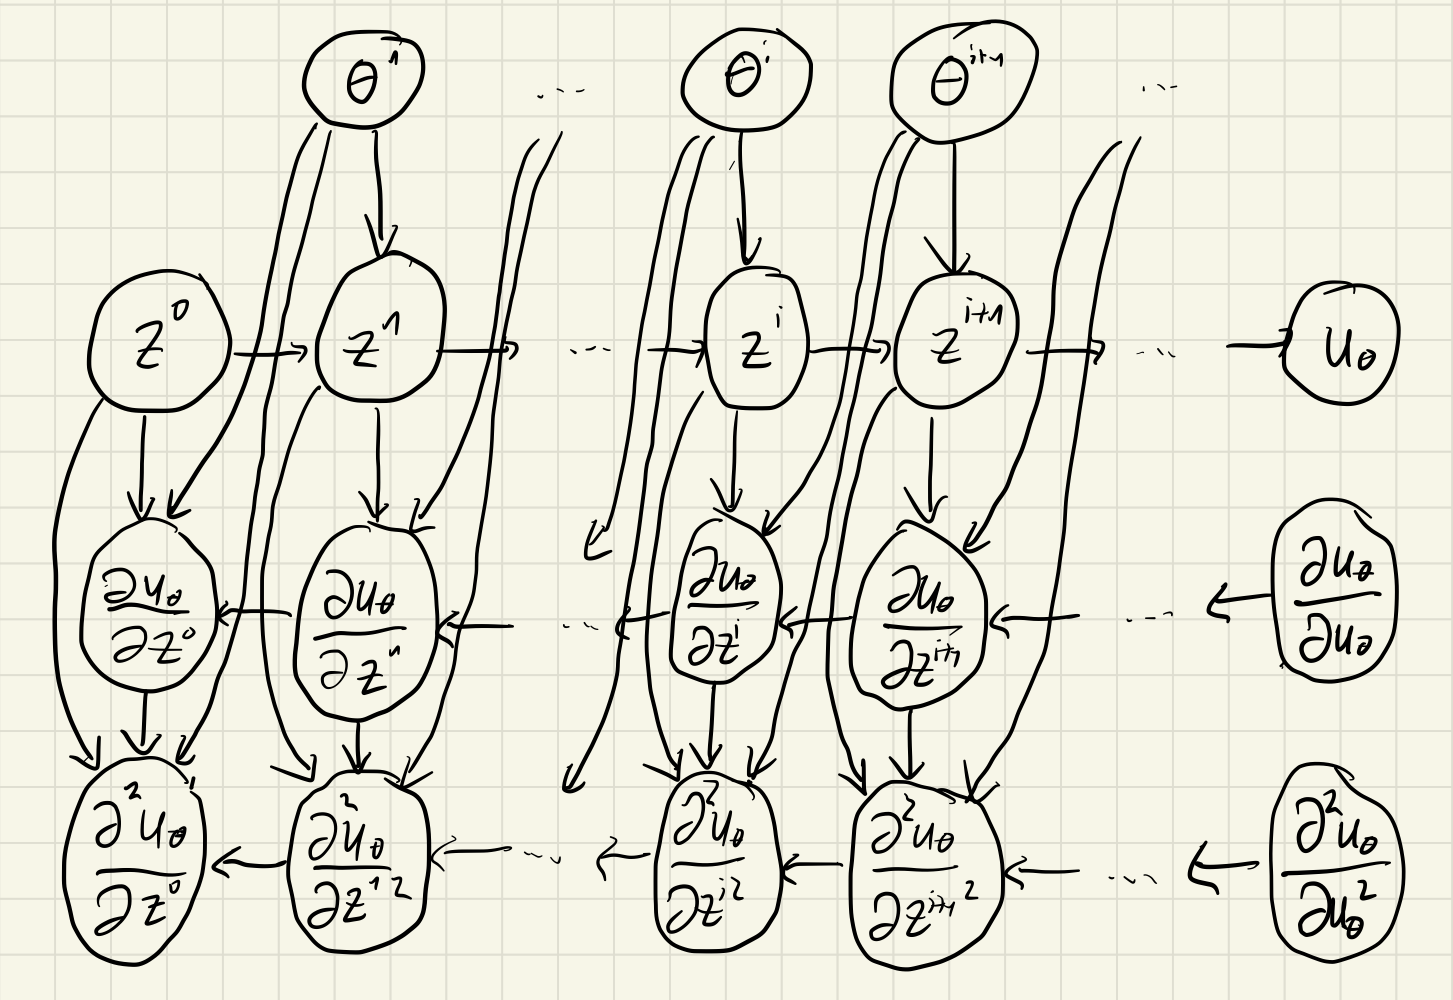
\includegraphics[width=0.6\linewidth]{figures/HBP_graph.png}
  \caption{Dependencies during gradient and Hessian backpropagation when computing the Hessian $\gradsquared{\vx}u_{\vtheta}$.}\label{fig:hbp-dependencies}
  \label{fig:hbp-dependencies}
\end{figure}

Following the procedure of \Cref{eq:hessian-backpropagation} yields the
per-layer parameter and feature Hessians $\gradsquared{\vz^{(i)}}u,
\gradsquared{\vtheta^{(i)}}u$. In \Cref{fig:hbp-dependencies} we depict the dependencies of
intermediate gradients and Hessians for computing $\gradsquared{\vx}u_{\vtheta}$:
\begin{itemize}
\item $\grad{\vz^{(i-1)}}u$ depends on $\grad{\vz^{(i)}}$ due to the recursion in \Cref{eq:gradient-backpropagation}, and on $\vz^{(i-1)}, \vtheta^{(i)}$ due to the Jacobian $\mJ_{\vz^{(i-1)}}\vz^{(i)}$ in the gradient backpropagation \Cref{eq:gradient-backpropagation}.

\item $\gradsquared{\vz^{(i-1)}}u$ depends on $\gradsquared{\vz^{(i)}}u$ and $\grad{\vz^{(i)}} u$ due to the recursion in \Cref{eq:hessian-backpropagation}, and on $\vz^{(i-1)}, \vtheta^{(i)}$ due to the Jacobian $\mJ_{\vz^{(i-1)}}\vz^{(i)}$ and Hessian $\gradsquared{\vz^{(i-1)}}[\vz^{(i)}]_k$ in the Hessian backpropagation \Cref{eq:gradient-backpropagation}.
\end{itemize}

%\subsection{Laplacian}

The Laplacian $\Delta u_{\vtheta}$ follows by taking the trace of
$\gradsquared{\vx}u_{\vtheta}$ from above, and is hence recursively defined.

\begin{figure}[t]
  \centering
  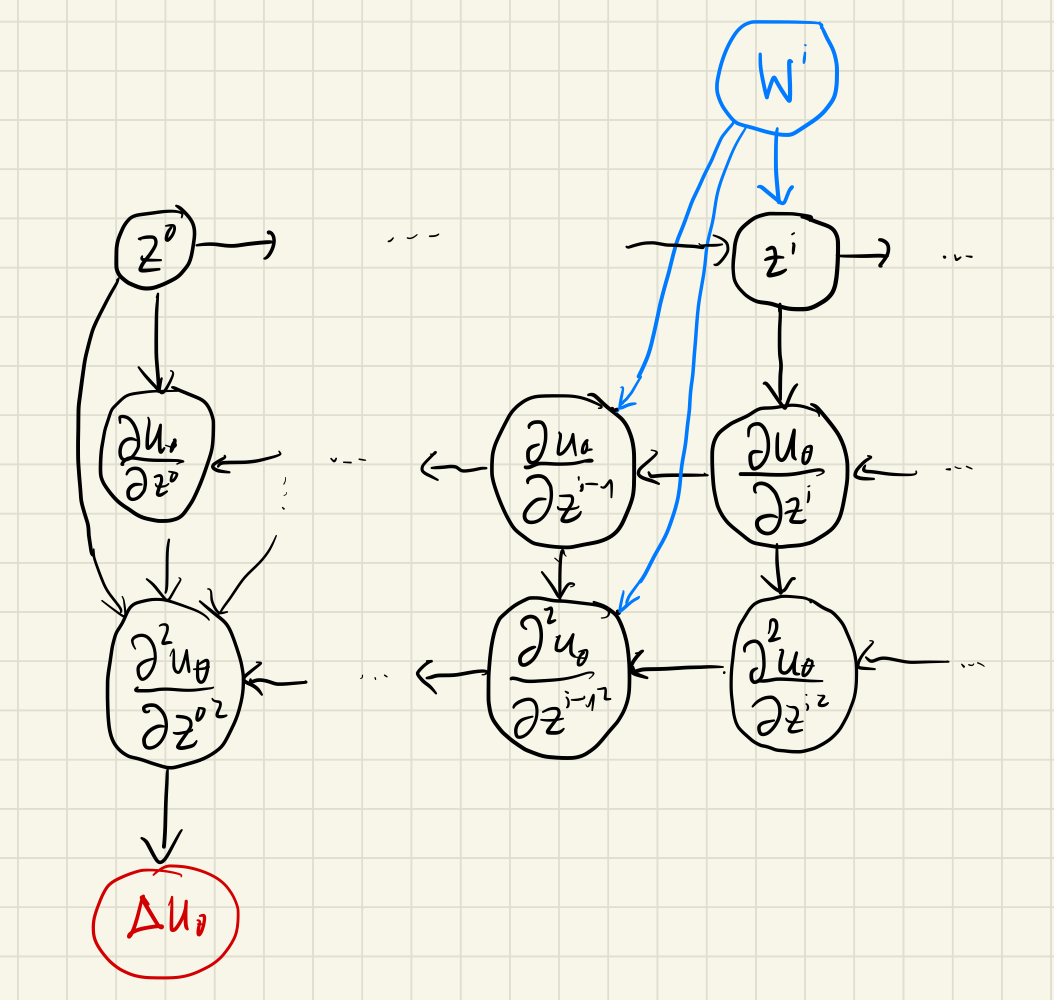
\includegraphics[width=0.6\linewidth]{figures/HBP_graph_weight.png}
  \caption{Direct children of the weight matrix of a single layer for the computation graph of the Laplacian.}\label{fig:laplacian-graph-weight}
\end{figure}

\paragraph{Hessian backpropagation through nonlinear layers}
We mostly consider nonlinear layers without trainable parameters and consist of a componentwise nonlinearity $z\mapsto \sigma(z)$ for some $\sigma\colon\mathbb R\to\mathbb R$ and we assume $\sigma$ to be twice continuously differentiable (I guess one ask for weaker things). 
The Jacobian of such a nonlinear layer is given by 
\begin{equation}
    \jac_{\vz^{(i-1)}}\vz^{(i)} = \operatorname{diag}(\sigma'(\vz^{(i-1)}))
\end{equation}
and the %Hessian acts as
%\begin{equation*}
%    (\nabla^2_{\vz^{(i-1)}\vz^{(i)})(u,v) = u\odot v\odot \sigma''(z). %u^\top \operatorname{diag}(\sigma''(\vz_{i-1}))v = (v\top)
%\end{equation*}
Hessian terms are given by
\begin{equation}
    \nabla^2_{\vz^{(i-1)}}[\vz^{(i)}]_k = \sigma''(\vz^{(i-1)}_k) e_k  e_k^\top.
\end{equation}
\toodoo{Someone should definitely double check}
With these two identities we can backpropogate the input Hessian through the non-trainable nonlinear layers and obtain
\begin{equation}
    \gradsquared{\vz^{(i-1)}}u
    =
      \left( \operatorname{diag}(\sigma'(\vz^{(i-1)})) \right)^{\top}
      \gradsquared{\vz^{(i)}}u
      \left( \operatorname{diag}(\sigma'(\vz^{(i-1)})) \right)
      +
      \sum_{k=1}^{h^{(i)}}
      \operatorname{diag}(\sigma''(\vz^{(i-1)_k})
      e_k e_k^\top
      [\grad{\vz^{(i)}} u]_k\,,
\end{equation}

\paragraph{Hessian backpropagation through a linear layer} To de-clutter the dependency graph of \Cref{fig:hbp-dependencies}, we will now consider the dependency of $\Delta u_{\vtheta}$ w.r.t.\,the weight of a single layer.
We assume this layer $i$ to be a linear layer with parameters $\mW^{(i)}$ such that $\vtheta^{(i)} = \flatten(\mW^{(i)})$,
\begin{align}
  \vz^{(i)} = \mW^{(i)} \vz^{(i-1)}\,.
\end{align}
For this layer, the second terms in \Cref{eq:hessian-backpropagation} disappears because the local Hessians are zero, that is $\gradsquared{\vz^{(i-1)}}[\vz^{(i)}]_k = \vzero$ and $\gradsquared{\mW^{(i)}}[\vz^{(i)}]_k = \vzero$.
Also, the Jacobians are $\jac_{\mW^{(i)}}\vz^{(i)} = {\vz^{(i-1)}}^{\top} \otimes \mI$ and $\jac_{\vz^{(i-1)}}\vz^{(i)} = \mW^{(i)}$ and hence only depends on one of the two layer inputs.
This simplifies the computation graph.
\Cref{fig:laplacian-graph-weight} shows the dependencies of $\mW^{(i)}$ on the
Laplacian, highlighting its three direct children,
\begin{align}\label{eq:spatialDerivatives}
  \begin{split}
    \vz^{(i)}
    &=
      \mW^{(i)} \vz^{(i-1)}
    \\
    \grad{\vz^{(i-1)}}u
    &=
      {\mW^{(i)}}^{\top}
      \left(
      \grad{\vz^{(i)}}u
      \right)
    \\
    \gradsquared{\vz^{(i-1)}}u
    &=
      {\mW^{(i)}}^{\top}
      \left(
      \gradsquared{\vz^{(i)}}u
      \right)
      \mW^{(i)}
  \end{split}
\end{align}

\subsection{Computing the parameter derivative of the input Laplacian} 
Recall, that the entries of the Fisher are composed from parameter derivatives of the input Laplacian, see~\eqref{eq:FisherInterior}. 
Here, we only consider architectures where only the linear layers possess trainable parameters and therefore we compute the parameter $\partial_{\theta} \Delta u_\theta$ of the input Laplacian. 

We have now identified the direct children of $\mW^{(i)}$ in the Laplacian's compute graph.
This allows us to write down its derivative $\grad{\mW^{(i)}} \Delta u$, which---by the chain rule---is simply the accumulated backpropagated error from the direct children:
\begin{align}\label{eq:laplacian-gradient}
  \begin{split}
    \grad{\mW^{(i)}} \Delta u_{\vtheta}
    &=
      \sum_{\bullet \in \left\{ \vz^{(i)}, \grad{\vz^{(i-1)}}u, \gradsquared{\vz^{(i-1)}}u \right\}}
      \left(
      \jac_{\mW^{(i)}}\bullet
      \right)^{\top}
      \grad{\bullet}\Delta u
    \\
    &=
      \left(
      \jac_{\mW^{(i)}}\vz^{(i)}
      \right)^{\top}
      \grad{\vz^{(i)}}\Delta u
      +
      \left(
      \jac_{\mW^{(i)}}\grad{\vz^{(i-1)}}u
      \right)^{\top}
      \grad{\grad{\vz^{(i-1)}}u}\Delta u
      +
      \left(
      \jac_{\mW^{(i)}}\gradsquared{\vz^{(i-1)}}u
      \right)^{\top}
      \grad{\gradsquared{\vz^{(i-1)}}u}\Delta u\,.
  \end{split}
\end{align}

%\paragraph{The Fisher} 
With the Laplacian's gradient \Cref{eq:laplacian-gradient}, we can write down the Fisher block (up to summation over the data) for $\mW^{(i)}$ as 
\begin{align}\label{eq:fisher}
  \begin{split}
    \mF^{(i)}
    &=
      \left(
      \grad{\mW^{(i)}} \Delta u_{\vtheta}
      \right)
      \left(
      \grad{\mW^{(i)}} \Delta u_{\vtheta}
      \right)^{\top}
    \\
    &=
      \sum_{\textcolor{blue}{\bullet} \in \left\{ \vz^{(i)}, \grad{\vz^{(i-1)}}u, \gradsquared{\vz^{(i-1)}}u \right\}}
      \sum_{\textcolor{red}{\bullet} \in \left\{ \vz^{(i)}, \grad{\vz^{(i-1)}}u, \gradsquared{\vz^{(i-1)}}u \right\}}
      \left(
      \left(
      \jac_{\mW^{(i)}}\textcolor{blue}{\bullet}
      \right)^{\top}
      \grad{\textcolor{blue}{\bullet}}\Delta u
      \right)
      \left(
      \left(
      \jac_{\mW^{(i)}}\textcolor{red}{\bullet}
      \right)^{\top}
      \grad{\textcolor{red}{\bullet}}\Delta u
      \right)^{\top}
    \\
    &=
      \sum_{\textcolor{blue}{\bullet} \in \left\{ \vz^{(i)}, \grad{\vz^{(i-1)}}u, \gradsquared{\vz^{(i-1)}}u \right\}}
      \sum_{\textcolor{red}{\bullet} \in \left\{ \vz^{(i)}, \grad{\vz^{(i-1)}}u, \gradsquared{\vz^{(i-1)}}u \right\}}
      \underbrace{
      \left(
      \jac_{\mW^{(i)}}\textcolor{blue}{\bullet}
      \right)^{\top}
      \left[
      \left(
      \grad{\textcolor{blue}{\bullet}}\Delta u
      \right)
      \left(
      \grad{\textcolor{red}{\bullet}}\Delta u
      \right)^{\top}
      \right]
      \left(
      \jac_{\mW^{(i)}}\textcolor{red}{\bullet}
      \right)}_{
      \coloneqq \mF^{(i)}_{\textcolor{blue}{\bullet}, \textcolor{red}{\bullet}}
      }\,.
  \end{split}
\end{align}

The Fisher consists of nine different terms.
Eventually, we would like to approximate it with a single Kronecker product, like KFAC~\citep{martens2015optimizing}. 
\toodoo{We could either work with the diagonal terms, or if all terms admit Kronecker representations we could also approximate this sum of Kroneckers by the Kronecker of the sums...?}
We begin by studying the diagonal terms $\mF_{\textcolor{blue}{\bullet}, \textcolor{blue}{\bullet}}^{(i)}$ and call them zeroth, first and second order diagonal terms for $\textcolor{blue}{\bullet} = \vz, \nabla u, \nabla^2 u$, respectively.
\toodoo{Other question: might it be possible to write the nine terms as a Kronecker product of a sum of 3 matrices with a sum of 3 matrices?}

\paragraph{Computing $\mJ_{\mW^{(i)}}\textcolor{blue}{\bullet}$} 
Let us first compute the Jacobians $\mJ_{\mW^{(i)}}\textcolor{blue}{\bullet}$ for which we envoke~\eqref{eq:spatialDerivatives}. 
We already know the Jacobian from the linear layer's forward pass,
\begin{subequations}\label{eq:fisher-jacobians}
  \begin{align}
    \jac_{\mW}\left( \mW \vx \right) = \vx^{\top} \otimes \mI\,.
  \end{align}
  The Jacobian from the gradient backpropagation is
  \begin{align}
    \jac_{\mW}\left( \mW^{\top} \vx \right) = \mI \otimes \vx^{\top}\,,
  \end{align}
  and the Jacobian from the Hessian backpropagation is
  \begin{align}
    \jac_{\mW}\left( \mW^{\top} \mX \mW \right) = \mI \otimes \mW^{\top}\mX + \mI \otimes \mW^{\top}\mX^{\top}\,.
  \end{align}
\end{subequations}
\toodoo{F.D.\,derived the Jacobians from \Cref{eq:fisher-jacobians} by hand.
  Might be worth to double-check for correctness.}

JM double checked and got the following:
Using the vec-trick~\eqref{eq:vecTrick} we obtain 
\[  \jac_{\mW}(\mW \vx) = \vx^\top\otimes \mI \]
and 
\[ \jac_\mW(\flatten(\mW^\top \vx)) = \jac_\mW(\flatten(\vx^\top\mW)^\top)) = \jac_\mW(K\flatten(\vx^\top\mW))) = K\jac_\mW(\flatten(\vx^\top\mW))) = K (\mI\otimes \vx^\top),  \]
where $K$ is the commutation matrix of the right dimensions, i.e., $K\flatten(A) = \flatten(A^\top)$. 
%I think this does not agree with $\mI\otimes \vx^\top$ as 
%Note that we need the commutation matrix
%\[ (\mI\otimes \vx) \]
Note that 
\[ (W+A)^\top X (W+A) - W^\top X W = W^\top X A + A^\top X W + O(\lVert A \rVert^2) \]
and hence 
\[ \jac_W(W^\top X W)A = . \]
By the vec-trick~\eqref{eq:vecTrick} we have $\flatten(\mW^\top\mX \mW) = (\mW^\top\otimes \mW^\top)\flatten(\mX)$ and hence 
\[ \jac_{\mW}\left( \mW^{\top} \mX \mW \right) = \mI \otimes (\mW^{\top}\mX) + K (\mI \otimes (\mW^{\top}\mX^{\top})). \]
\toodoo{Ok, I thought this made sense, but now it confuses me...}


The Jacobians from \Cref{eq:fisher-jacobians} allow to express the Fisher in
terms of Kronecker-structured expressions consisting of 16 terms in total.

\toodoo{F.D.\,Write down the full expression for the Fisher.
  Propose ways to Kronecker-approximate each of the 16 terms, such that we end up with a single Kronecker product in the end.}

Overall, with~\eqref{eq:spatialDerivatives} this yields 
\begin{align}
  \begin{split}
    \jac_{\mW^{(i)}}\vz^{(i)}
    &=
      {\vz^{(i-1)}}^\top\otimes I
    \\
    \jac_{\mW^{(i)}}\grad{\vz^{(i-1)}}u
    &=
      I\otimes 
      \grad{\vz^{(i)}}u
    \\
    \jac_{\mW^{(i)}}\gradsquared{\vz^{(i-1)}}u
    &=
    \mI \otimes (\mW^{\top}\gradsquared{\vz^{(i)}}u) + K (\mI \otimes (\mW^{\top}(\gradsquared{\vz^{(i)}}u)^{\top}))
  \end{split}
\end{align}


\paragraph{Computing $\grad{\textcolor{blue}{\bullet}}\Delta u$}
In order to evaluate the Fisher we also need to compute the terms $\grad{\textcolor{blue}{\bullet}}\Delta u$ for all children, more specifically $\grad{\vz^{(i)}}\Delta u$, $\grad{\grad{\vz^{(i-1)}}u}\Delta u$ and $\grad{\gradsquared{\vz^{(i-1)}}u}\Delta u$.
\toodoo{DO we need to understand how we compute this? We can definitely do this via backprop, but then additional terms would appear I guess}


\paragraph{Zeroth order diagonal term}
Note that one of the nine terms is the term similar to the original KFAC paper, namely
when $\textcolor{blue}{\bullet} = \textcolor{red}{\bullet} = \vz^{(i)}$
(remember that $\jac_{\mW^{(i)}} \vz^{(i)} = \vz^{(i-1)} \otimes \mI$):
\begin{align}\label{eq:original-kfac}
  \begin{split}
    \mF^{(i)}_{\textcolor{blue}{\vz^{(i)}}, \textcolor{red}{\vz^{(i)}}}
    &=
      \left(
      \textcolor{blue}{\vz^{(i-1)} \otimes \mI}
      \right)
      \left[
      \left(
      \textcolor{blue}{\grad{\vz^{(i-1)}}\Delta u}
      \right)
      \left(
      \textcolor{red}{\grad{\vz^{(i-1)}}\Delta u}
      \right)^{\top}
      \right]
      \left(
      \textcolor{red}{{\vz^{(i-1)}}^{\top} \otimes \mI}
      \right)
    \\
    &=
      \textcolor{blue}{\vz^{(i-1)}}
      \textcolor{red}{{\vz^{(i-1)}}^{\top}}
      \otimes
      \left(
      \textcolor{blue}{\grad{\vz^{(i-1)}}\Delta u}
      \right)
      \left(
      \textcolor{red}{\grad{\vz^{(i-1)}}\Delta u}
      \right)^{\top}
    \\
    &\coloneqq \mA_{\text{KFAC}}^{(i)} \otimes \mB_{\text{KFAC}}^{(i)}\,.
  \end{split}
\end{align}
\toodoo{I think the subscript should be $\nabla_{\vz^{(i)}} \Delta u$ instead of $\nabla_{\vz^{(i-1)}} \Delta u$ or am I missing something? }
Note however, that in comparison to traditional KFAC, there are Laplacian terms. 
\Cref{eq:original-kfac} illustrates that the Kronecker structure emerges from
the Jacobians. So we need to investigate these objects closer for the remaining
terms of \Cref{eq:fisher}.


\paragraph{First order diagonal term}

\paragraph{Second order diagonal term}


%%% Local Variables:
%%% mode: latex
%%% TeX-master: "../main"
%%% End:
